Zur Bereicherung der Freizeit wird vom Sportinstitut der Universität jedes
Semester ein breitgefächertes Programm von Sportkursen
angeboten\footnote{\url{http://www.hsp.uni-tuebingen.de/}}. Diese Kurse sind
meist auf Einsteigerniveau und eignen sich bestens, um eine Sportart einfach
mal auszuprobieren.\\
Die meisten Kurse finden in den Hallen des Sportinstituts (Wilhelmstraße,
Alberstraße) statt, teilweise werden aber auch Exkursionen angeboten.\\
Die Teilnahme ist für Studierende meist relativ günstig, weshalb die Kursplätze
schnell belegt sind. Wenn man sich für einen Kurs anmelden möchte, sollte man
auf jeden Fall den auf der Website ausgeschriebenen Anmeldestart beachten und
sich zeitnah anmelde. In den letzten Semestern waren die Server für die
Anmeldung bereits 10 Minuten vor Anmeldungsbeginn komplett überlastet, 5
Minuten nach Anmeldungsbeginn waren alle Plätze vergriffen. Sucht euch also,
wenn ihr unbedingt in einen Kurs wollt, für die Anmeldung einen Platz mit guter
Internetanbindung an die Uni-Server ;)

\textbf{Vorsicht:} Im Umkleidebereich wird "`traditionell"' extrem viel
  geklaut, also Uhr, Portemonnaie und am besten auch das Smartphone gleich
  zu Hause lassen und die Sporttasche wäh\-rend des Trainings in
  die Halle mitnehmen. Den Studentenausweis solltet ihr jedoch immer dabei haben, 
  denn der wird ab und zu am Eingang kontrolliert.
 
\vfill

\begin{center}
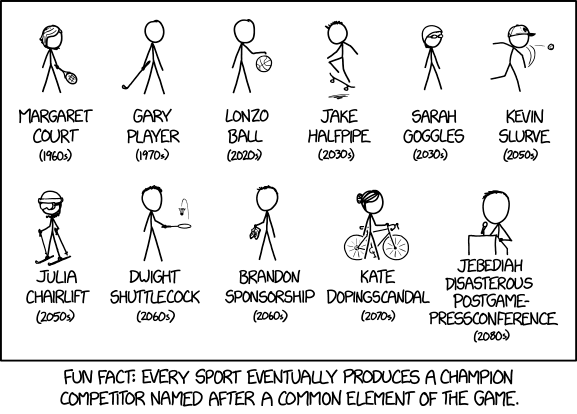
\includegraphics[width=0.8\hsize]{info/xkcd/sports_champions.png}
\end{center}
